\documentclass[tikz,border=8pt]{standalone}

\usepackage{amsmath,amssymb}
\usepackage{tikz}
\usetikzlibrary{arrows.meta, positioning, calc, fit, backgrounds, shapes.geometric}

% ============================================================
% COLORS
% ============================================================
% stage fills are given as OPAQUE pre-blended colours (instead of
% fill opacity) so that a line can be given a halo in exactly the
% background colour -- this is what makes the one unavoidable
% line crossing render as a clean "hop" instead of a junction.
\definecolor{s1fill}{RGB}{248,251,255}
\definecolor{s2fill}{RGB}{249,253,249}

\definecolor{semantic}{RGB}{229,224,250}
\definecolor{detail}{RGB}{218,246,228}
\definecolor{latent}{RGB}{255,244,210}
\definecolor{vq}{RGB}{244,232,255}
\definecolor{flow}{RGB}{255,231,222}
\definecolor{attention}{RGB}{224,239,255}
\definecolor{decoder}{RGB}{231,236,255}

\definecolor{blueDark}{RGB}{25,73,115}
\definecolor{greenDark}{RGB}{35,120,78}
\definecolor{purpleDark}{RGB}{105,70,145}
\definecolor{redDark}{RGB}{145,65,55}

% ============================================================
% STYLES
% ============================================================
\tikzset{
    >=Latex,
    arrow/.style={->, line width=0.8pt, shorten >=1.5pt, shorten <=1.5pt},
    line/.style={line width=0.8pt},
    dashedarrow/.style={->, dashed, line width=0.8pt, shorten >=1.5pt, shorten <=1.5pt},
    % a solid arrow that "hops" over whatever it crosses
    hoparrow/.style={arrow, preaction={draw, line width=3.4pt, s1fill}},
    junction/.style={circle, fill=black, inner sep=0pt, minimum size=3.4pt},
    stage1/.style={rounded corners=9pt, draw=blue!45, dashed, line width=1pt, fill=s1fill},
    stage2/.style={rounded corners=9pt, draw=green!45!black, dashed, line width=1pt, fill=s2fill},
    input/.style={rounded corners=5pt, draw=black!60, fill=white, minimum width=1.5cm, minimum height=.9cm, align=center, font=\small},
    semantic/.style={rounded corners=6pt, draw=blue!60!black, fill=semantic, minimum width=3.6cm, minimum height=1.1cm, align=center, font=\small},
    detail/.style={rounded corners=6pt, draw=green!60!black, fill=detail, minimum width=3.6cm, minimum height=1.1cm, align=center, font=\small},
    latent/.style={rounded corners=5pt, draw=orange!65!black, fill=latent, minimum width=1.3cm, minimum height=.65cm, align=center, font=\small},
    vq/.style={rounded corners=5pt, draw=purpleDark, fill=vq, minimum width=1.8cm, minimum height=.85cm, align=center, font=\small},
    transformerbox/.style={rounded corners=7pt, draw=redDark, fill=flow, align=center},
    attn/.style={rounded corners=4pt, draw=blue!60!black, fill=attention, minimum width=2.7cm, minimum height=.65cm, align=center, font=\scriptsize},
    decoder/.style={rounded corners=6pt, draw=blue!55!black, fill=decoder, minimum width=1.7cm, minimum height=.85cm, align=center, font=\small}
}

% stage frames need their own layer: they must sit behind the
% STDiT box, which is itself on the background layer
\pgfdeclarelayer{stagebg}
\pgfsetlayers{stagebg,background,main}

\begin{document}
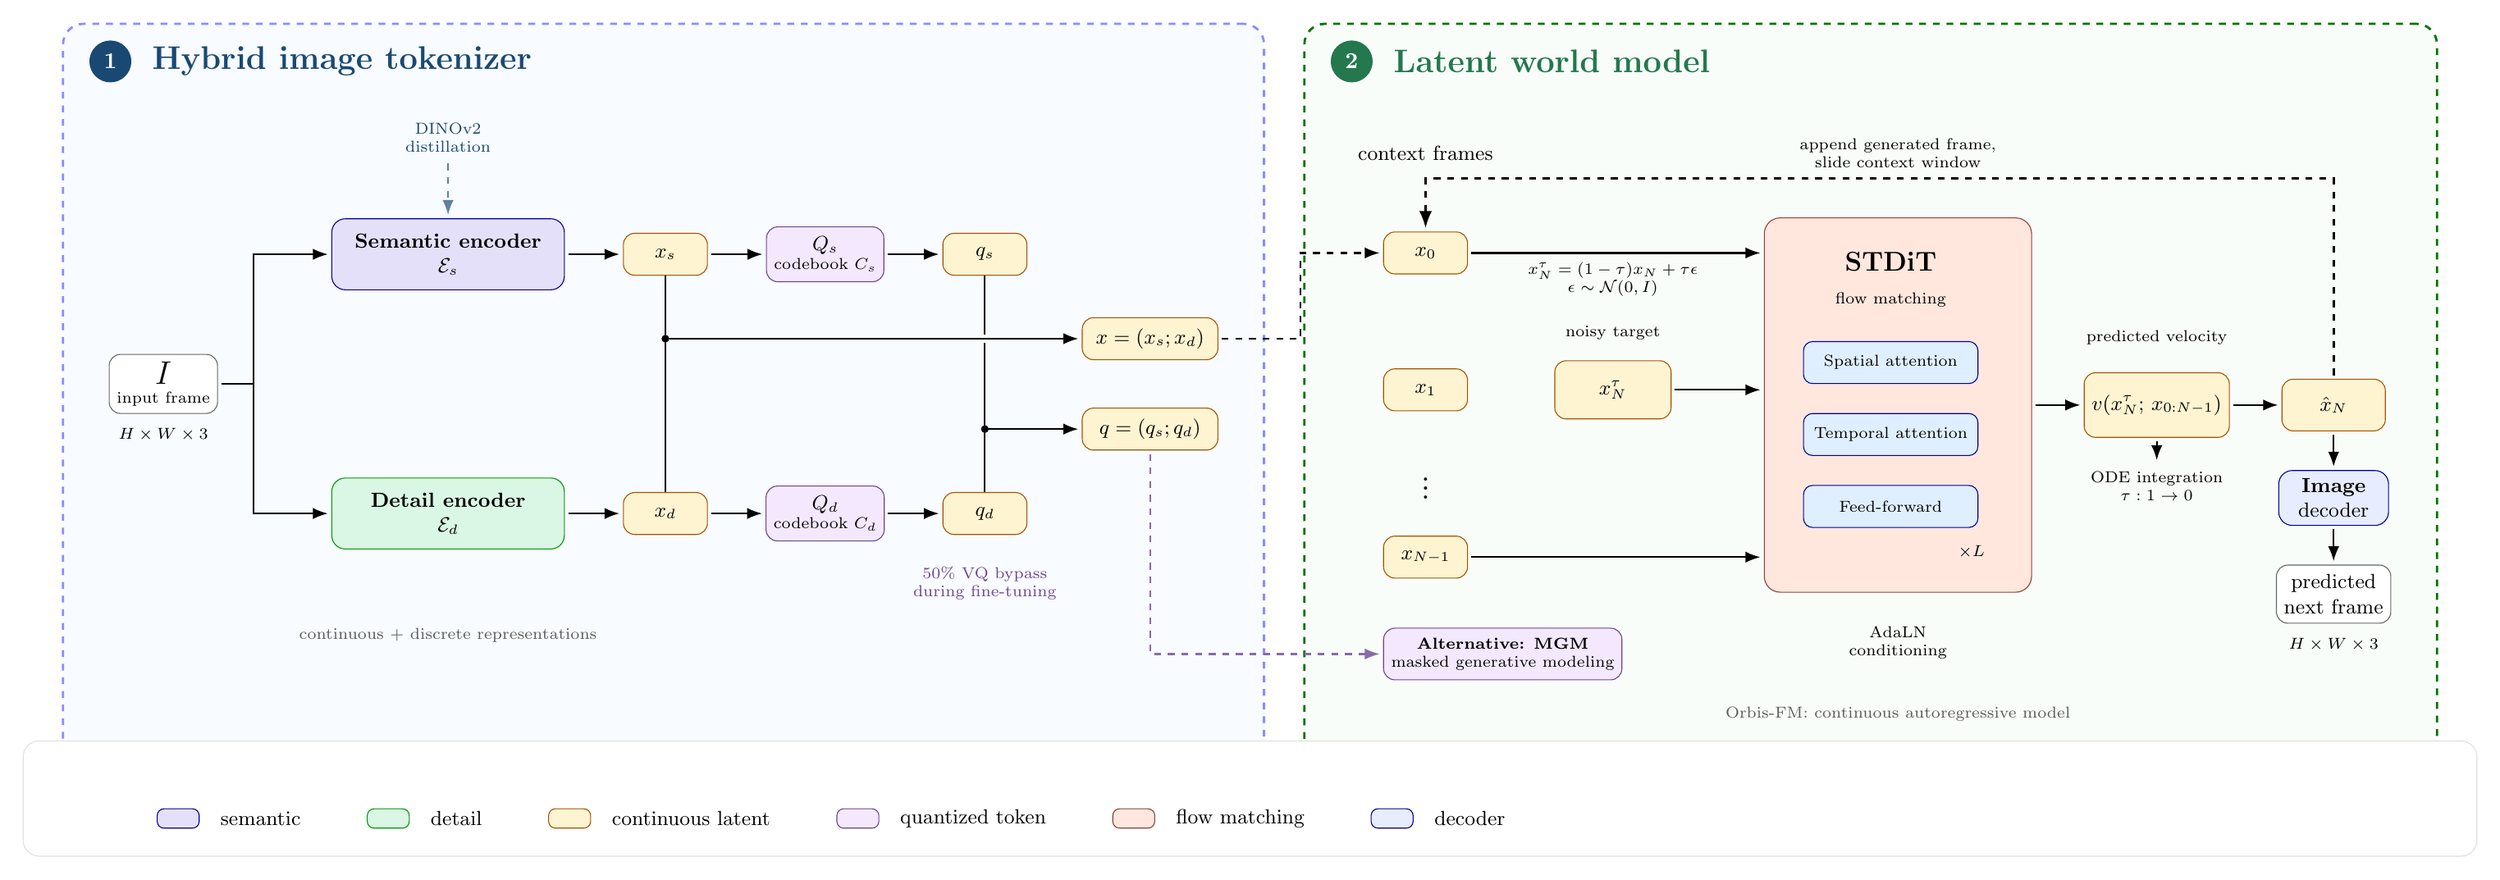
\begin{tikzpicture}

% ############################################################
% STAGE 1 CONTENT
% ############################################################

\node[semantic] (Es) {\textbf{Semantic encoder}\\$\mathcal E_s$};
\node[detail, below=2.9cm of Es] (Ed) {\textbf{Detail encoder}\\$\mathcal E_d$};
\coordinate (rowMid) at ($(Es)!0.5!(Ed)$);

% ---- input frame: pushed further left so BOTH trunk arrows have
% a clearly visible horizontal run before they branch ----
\coordinate (Ipos) at ($(Es.west)+(-2.6,0)$);
\node[input] (I) at (Ipos |- rowMid) {\Large $I$\\[-1mm]\scriptsize input frame};
\node[below=1mm of I, font=\scriptsize] (Ilabel) {$H\times W\times3$};

% step east first, THEN branch: the vertical riser sits in open
% space rather than hugging the box edge
\draw[arrow] (I.east) -- ++(0.55,0) |- (Es.west);
\draw[arrow] (I.east) -- ++(0.55,0) |- (Ed.west);

\node[align=center, font=\scriptsize, text=blueDark, above=9mm of Es] (dino) {DINOv2\\distillation};
\draw[dashedarrow, blueDark!70] (dino.south) -- (Es.north);

\node[latent, right=9mm of Es] (xs) {$x_s$};
\node[latent] (xd) at (xs |- Ed) {$x_d$};
\draw[arrow] (Es.east) -- (xs.west);
\draw[arrow] (Ed.east) -- (xd.west);

\node[vq, right=9mm of xs] (Qs) {$Q_s$\\[-1mm]\scriptsize codebook $C_s$};
\node[vq] (Qd) at (Qs |- Ed) {$Q_d$\\[-1mm]\scriptsize codebook $C_d$};
\draw[arrow] (xs.east) -- (Qs.west);
\draw[arrow] (xd.east) -- (Qd.west);

\node[latent, right=9mm of Qs] (qs) {$q_s$};
\node[latent] (qd) at (qs |- Ed) {$q_d$};
\draw[arrow] (Qs.east) -- (qs.west);
\draw[arrow] (Qd.east) -- (qd.west);

% ---- concatenation outputs -------------------------------------
% Both are reached by a single arrow tapped off a vertical
% "concat bus", so each output node has exactly ONE arrowhead
% entering it, dead-centre on its west edge. This is what fixes
% the doubled / misaligned arrows out of x_s and x_d.
\coordinate (outX)  at ($(qs.east)+(1.9,0)$);
\coordinate (xRowY) at ($(rowMid)+(0,0.7)$);
\coordinate (qRowY) at ($(rowMid)+(0,-0.7)$);

\node[latent, minimum width=2.1cm] (xcomb) at (outX |- xRowY) {$x=(x_s;x_d)$};
\node[latent, minimum width=2.1cm] (qcomb) at (outX |- qRowY) {$q=(q_s;q_d)$};

% concat buses (plain lines: they denote joining, not flow)
\draw[line] (xs.south) -- (xd.north);
\draw[line] (qs.south) -- (qd.north);

\coordinate (xtap) at (xs |- xcomb);
\coordinate (qtap) at (qs |- qcomb);
\node[junction] at (xtap) {};
\node[junction] at (qtap) {};

% the x tap-off is the only line in the figure that must cross
% another; the halo makes it hop cleanly over the q bus
\draw[hoparrow] (xtap) -- (xcomb.west);
\draw[arrow]    (qtap) -- (qcomb.west);

\node[font=\scriptsize, text=purpleDark, align=center] (bypasslabel)
    at ($(qd.south)+(0,-0.75)$) {50\% VQ bypass\\during fine-tuning};
\node[font=\scriptsize, text=gray!70!black, below=1.1cm of Ed] (contcaption)
    {continuous + discrete representations};

\coordinate (s1TitleSpacer) at ($(dino.north)+(0,0.9)$);

% invisible fit over stage-1 content only (used to anchor stage 2
% and, later, to draw the visible stage-1 frame)
\node[fit=(Es)(Ed)(I)(Ilabel)(dino)(xs)(xd)(Qs)(Qd)(qs)(qd)
          (xcomb)(qcomb)(bypasslabel)(contcaption)(s1TitleSpacer),
      inner sep=0pt, draw=none] (S1raw) {};

% ############################################################
% STAGE 2 CONTENT   (all anchored off S1raw, then chained)
% ############################################################

\coordinate (contextX) at ($(S1raw.east)+(3.2,0)$);
\coordinate (noisyX)   at ($(contextX)+(2.9,0)$);
\coordinate (stditX)   at ($(noisyX)+(4.3,0)$);
\coordinate (stditTopY) at ($(rowMid)+(0,1.9)$);

% ---- STDiT stack, box fitted to its own contents ----
\node[font=\bfseries\large] (stdit-title) at (stditX |- stditTopY) {STDiT};
\node[font=\scriptsize, below=1mm of stdit-title] (stdit-sub) {flow matching};
\node[attn, below=4mm of stdit-sub] (SA) {Spatial attention};
\node[attn, below=4.5mm of SA] (TA) {Temporal attention};
\node[attn, below=4.5mm of TA] (FF) {Feed-forward};
\node[font=\scriptsize, below=1.5mm of FF, xshift=1.25cm] (xL) {$\times L$};

\begin{scope}[on background layer]
\node[transformerbox, fit=(stdit-title)(stdit-sub)(SA)(TA)(FF)(xL),
      inner xsep=6mm, inner ysep=4mm] (STDiT) {};
\end{scope}

\node[font=\scriptsize, align=center, below=4mm of STDiT] (adaln) {AdaLN\\conditioning};

% ---- context frames, pinned to STDiT's own top/bottom ----
\coordinate (x0Y)   at ($(STDiT.north)+(0,-0.55)$);
\coordinate (xNm1Y) at ($(STDiT.south)+(0,0.55)$);

\node[latent] (x0)   at (contextX |- x0Y)   {$x_0$};
\node[latent] (xNm1) at (contextX |- xNm1Y) {$x_{N-1}$};
\coordinate (x1Y)    at ($(x0)!0.45!(xNm1)$);
\node[latent] (x1)   at (contextX |- x1Y)   {$x_1$};
\coordinate (vdotsY) at ($(x1)!0.55!(xNm1)$);
\node[font=\Large] (vdots) at (contextX |- vdotsY) {$\vdots$};

% ---- noisy target ----
\node[latent, minimum width=1.8cm, minimum height=.9cm] (xtau) at (noisyX |- x1Y) {$x_N^\tau$};
\node[font=\scriptsize, above=2mm of xtau] (noisylbl) {noisy target};
\node[align=center, font=\scriptsize, above=2mm of noisylbl] (equation)
    {$x_N^\tau=(1-\tau)x_N+\tau\epsilon$\\$\epsilon\sim\mathcal N(0,I)$};

\draw[arrow] (x0.east)   -- (STDiT.west |- x0.east);
\draw[arrow] (xNm1.east) -- (STDiT.west |- xNm1.east);
\draw[arrow] (xtau.east) -- (STDiT.west |- xtau.east);

% ---- velocity / xhat / decoder / output ----
\node[latent, minimum width=2.0cm, minimum height=1.0cm, right=8mm of STDiT] (v) {$v(x_N^\tau;\,x_{0:N-1})$};
\draw[arrow] (STDiT.east) -- (v.west);
\node[font=\scriptsize, above=3mm of v] (predvel) {predicted velocity};

\node[align=center, font=\scriptsize, below=4mm of v] (ode) {ODE integration\\$\tau:1\rightarrow0$};
\draw[arrow] (v.south) -- (ode.north);

\node[latent, minimum width=1.6cm, minimum height=.8cm, right=8mm of v] (xhat) {$\hat{x}_N$};
\draw[arrow] (v.east) -- (xhat.west);

\node[decoder, below=6mm of xhat] (D) {\textbf{Image}\\decoder};
\draw[arrow] (xhat.south) -- (D.north);

\node[input, minimum width=1.7cm, minimum height=.9cm, below=6mm of D] (out) {predicted\\next frame};
\draw[arrow] (D.south) -- (out.north);
\node[below=1mm of out, font=\scriptsize] (outlabel) {$H\times W\times3$};

% ---- autoregressive feedback, in a lane tied to STDiT's top edge ----
\coordinate (feedbackY) at ($(STDiT.north)+(0,0.6)$);
\draw[dashedarrow, line width=1pt]
    (xhat.north) -- (xhat |- feedbackY) -- (x0 |- feedbackY) -- (x0.north);

\node[font=\scriptsize, align=center] (appendlbl) at ($(STDiT |- feedbackY)+(0,0.4)$)
    {append generated frame,\\slide context window};
\node[font=\small] (ctxlabel) at ($(x0 |- feedbackY)+(0,0.4)$) {context frames};

% ---- discrete alternative: west-anchored on the context column so
% it cannot stick out to the left and collide with stage 1 ----
\node[rounded corners=5pt, draw=purpleDark, fill=vq, minimum height=.8cm,
      align=center, font=\scriptsize, anchor=west] (MGM) at ($(xNm1.west)+(0,-1.5)$)
    {\textbf{Alternative: MGM}\\masked generative modeling};

\node[font=\scriptsize, text=gray!70!black, below=5mm of adaln] (orbisfm)
    {Orbis-FM: continuous autoregressive model};

\coordinate (s2TitleSpacer) at ($(appendlbl.north)+(0,0.9)$);

\node[fit=(ctxlabel)(x0)(x1)(vdots)(xNm1)(equation)(noisylbl)(xtau)(STDiT)(adaln)
          (v)(predvel)(ode)(xhat)(D)(out)(outlabel)(MGM)(orbisfm)(appendlbl)(s2TitleSpacer),
      inner sep=0pt, draw=none] (S2raw) {};

% ---- cross-stage connectors (drawn after both stages exist) ----
\coordinate (elbowX) at ($(xcomb.east)!0.5!(x0.west)$);
\draw[dashedarrow] (xcomb.east) -- (elbowX |- xcomb) -- (elbowX |- x0) -- (x0.west);
\draw[dashedarrow, purpleDark!80] (qcomb.south) |- (MGM.west);

% ############################################################
% STAGE FRAMES -- forced to a COMMON top and bottom edge, and
% separated horizontally, so the two boxes are aligned and can
% never intersect.
% ############################################################

\node[fit=(S1raw)(S2raw), inner sep=0pt, draw=none] (ALL) {};
\coordinate (frameTop) at ($(ALL.north)+(0,0.5)$);
\coordinate (frameBot) at ($(ALL.south)+(0,-0.5)$);

\begin{pgfonlayer}{stagebg}
\node[stage1, fit=(S1raw)(S1raw.north |- frameTop)(S1raw.south |- frameBot),
      inner xsep=7mm, inner ysep=0pt] (S1) {};
\node[stage2, fit=(S2raw)(S2raw.north |- frameTop)(S2raw.south |- frameBot),
      inner xsep=7mm, inner ysep=0pt] (S2) {};
\end{pgfonlayer}

\node[circle, draw=blueDark, fill=blueDark, text=white, minimum size=.62cm, font=\bfseries]
    (badge1) at ($(S1.north west)+(0.75,-0.6)$) {1};
\node[anchor=west, font=\bfseries\Large, text=blueDark, right=2mm of badge1]
    {Hybrid image tokenizer};

\node[circle, draw=greenDark, fill=greenDark, text=white, minimum size=.62cm, font=\bfseries]
    (badge2) at ($(S2.north west)+(0.75,-0.6)$) {2};
\node[anchor=west, font=\bfseries\Large, text=greenDark, right=2mm of badge2]
    {Latent world model};

% ############################################################
% LEGEND
% ############################################################

\node[rounded corners=3pt, draw=blue!60!black, fill=semantic, minimum width=.65cm, minimum height=.3cm]
    (leg1) at ($(S1.south west)+(1.8,-0.85)$) {};
\node[anchor=west, font=\small, right=2mm of leg1] (leg1t) {semantic};

\node[rounded corners=3pt, draw=green!60!black, fill=detail, minimum width=.65cm, minimum height=.3cm,
      right=9mm of leg1t] (leg2) {};
\node[anchor=west, font=\small, right=2mm of leg2] (leg2t) {detail};

\node[rounded corners=3pt, draw=orange!65!black, fill=latent, minimum width=.65cm, minimum height=.3cm,
      right=9mm of leg2t] (leg3) {};
\node[anchor=west, font=\small, right=2mm of leg3] (leg3t) {continuous latent};

\node[rounded corners=3pt, draw=purpleDark, fill=vq, minimum width=.65cm, minimum height=.3cm,
      right=9mm of leg3t] (leg4) {};
\node[anchor=west, font=\small, right=2mm of leg4] (leg4t) {quantized token};

\node[rounded corners=3pt, draw=redDark, fill=flow, minimum width=.65cm, minimum height=.3cm,
      right=9mm of leg4t] (leg5) {};
\node[anchor=west, font=\small, right=2mm of leg5] (leg5t) {flow matching};

\node[rounded corners=3pt, draw=blue!55!black, fill=decoder, minimum width=.65cm, minimum height=.3cm,
      right=9mm of leg5t] (leg6) {};
\node[anchor=west, font=\small, right=2mm of leg6] (leg6t) {decoder};

\begin{pgfonlayer}{stagebg}
\node[rounded corners=7pt, draw=black!12, fill=white,
      fit=(leg1)(leg6t)(S1.south west)(S2.south east),
      inner xsep=6mm, inner ysep=3.5mm] (legend) {};
\end{pgfonlayer}

\end{tikzpicture}
\end{document}